 \section{Durchführung}
\label{sec:Durchführung}

\subsection{Gedämpfte Schwingungen}
\label{sec:durchgedschw}

Aufgabe ist es in diesem Abschnitt der Messung die Abklingzeit der gedämpften
Schwingung zu bestimmen und dann den effektiven Dämpfungswiderstand $R_{\text{eff}}$
zu berechnen.
Der Versuchsaufbau ist in Abbildung \ref{fig:schalta} zu sehen.

%schaltung a hier
\begin{figure}[h]
  \centering
  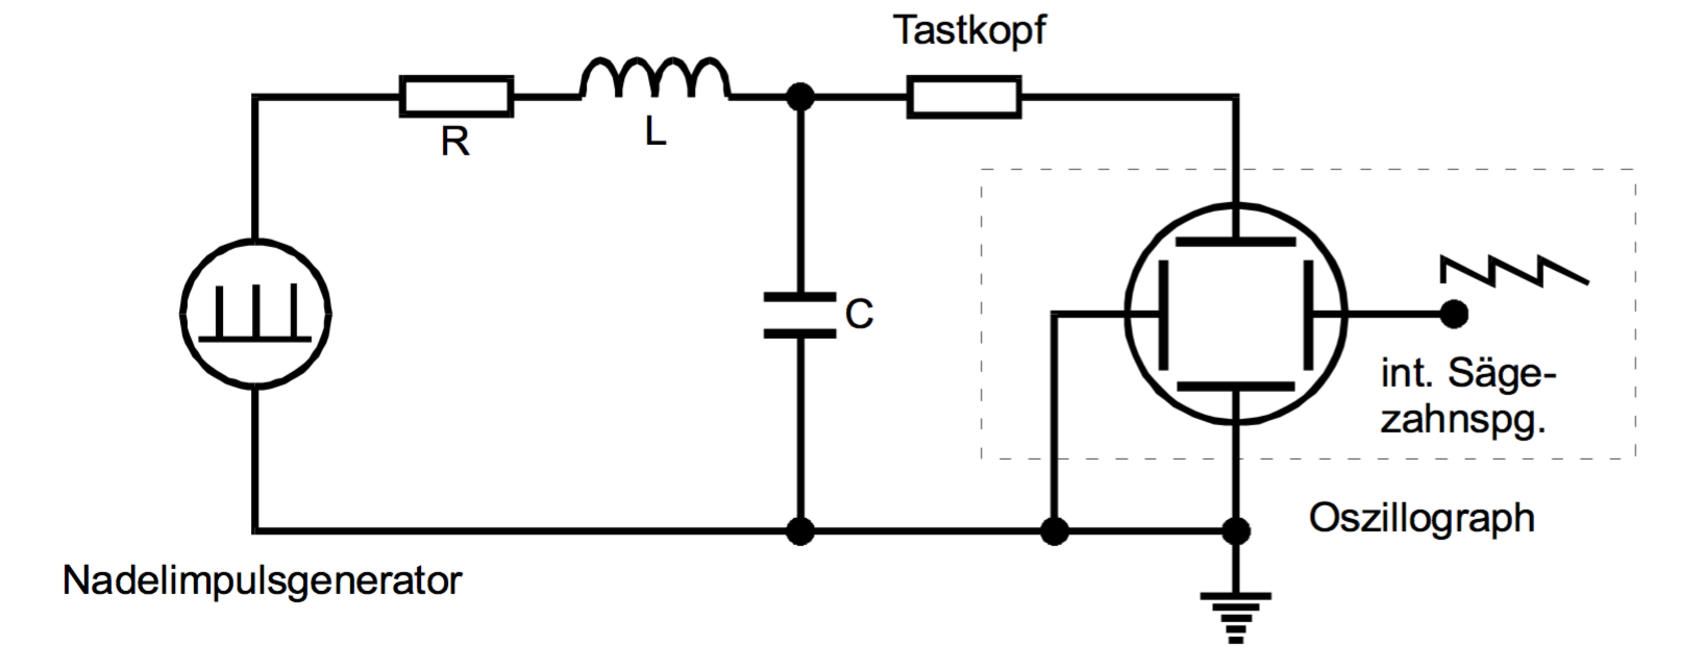
\includegraphics[width = \textwidth]{Schaltunga.pdf}
  \caption{Schaltung zur Bestimmung des effektiven Dämpfungswiderstands \cite{anleitung}.}
  \label{fig:schalta}
\end{figure}

Als Widerstand wird $R~=~\SI{682 +- 1}{\ohm}$ benutzt. Die Spule hat
die Impedanz $L~=~\SI{16.78 +- 0.09}{\milli\henry}$, der Kondensator besitzt
den Wert $C~=~\SI{2.066 +- 0.006}{\nano\farad}$.

Die Spannungsquelle liefert eine Rechteckspannung. Abgegriffen wird diese,
wie dargestellt, mit einem Tastkopf, der einen hohen Innenwiderstand
$R_{\text{i}}~=~\SI{10}{\mega\ohm}$ hat. Dann werden die Werte dem digitalen
Oszilloskop mit einem USB-Stick entnommen.

\subsection{Aperiodischer Grenzfall}

Nun wird der Widerstand $R_{\text{ap}}$ bestimmt, bei dem das Oszilloskop
eine exponentielle Abnahme der Spannung anzeigt.

%schaltung b hier
\begin{figure}[h]
  \centering
  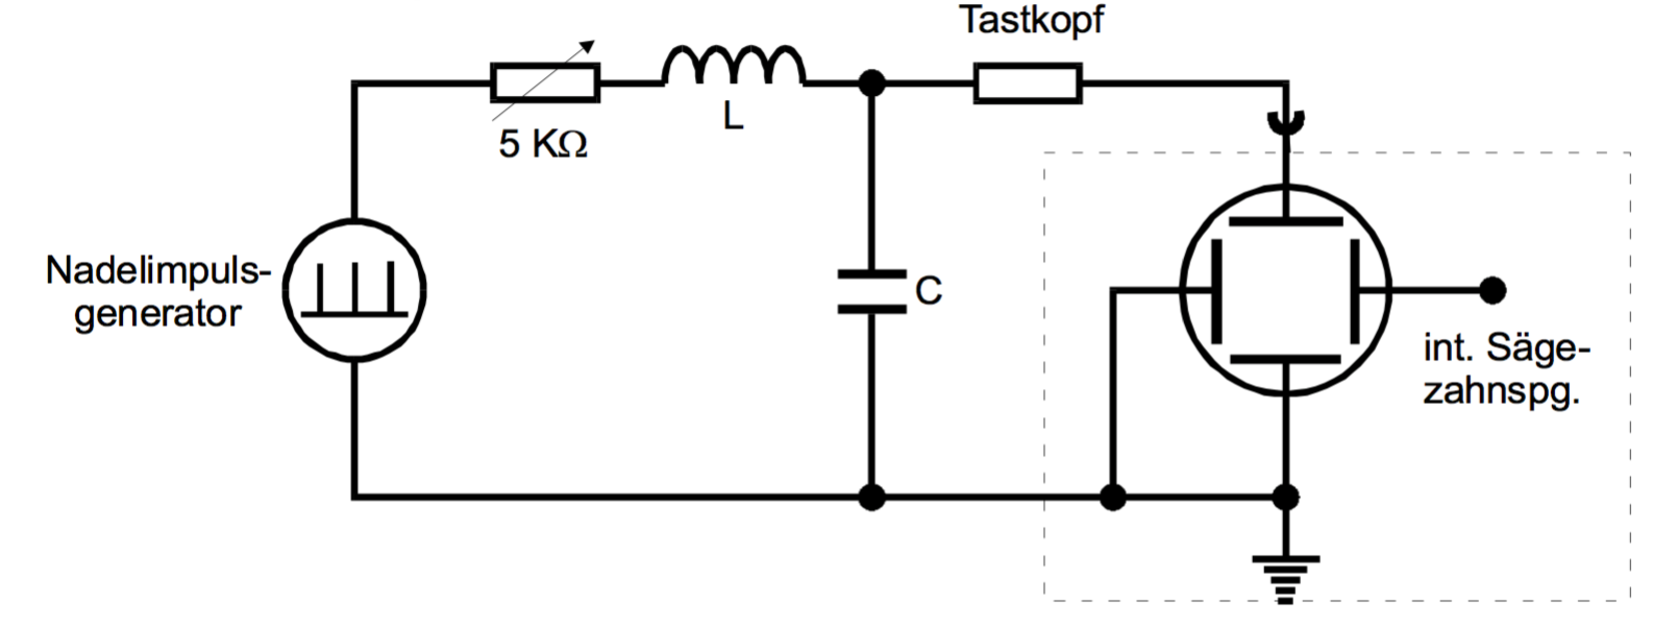
\includegraphics[width = \textwidth]{Schaltungb.pdf}
  \caption{Schaltung zur Bestimmung von $R_{\text{ap}}$ \cite{anleitung}.}
  \label{fig:schaltb}
\end{figure}

In Abbildung \ref{fig:schaltb} ist zu erkennen, dass ein ähnlicher
Versuchsaufbau wie in Kapitel \ref{sec:durchgedschw} benutzt wird.
Die oben erwähnten Bauteile sind die Selben und haben auch die selben Werte.
Nur der Widerstand $R$ ist in diesem Falle regelbar bis zu einem Maximum
von $\SI{5}{\kilo\ohm}$.

Um $R_{\text{ap}}$ zu finden wird er auf die maximalen $\SI{5}{\kilo\ohm}$
eingestellt und dann verringert, bis ein Überschwingen der Kurve auf dem
Schirm des Oszillographen zu beobachten ist. Dann wird $R$ wieder etwas
vergrößert, bis die Überschwingung verschwindet. $R_{\text{ap}}$ ist dann
gefunden und wird notiert.

\subsection{Erzwungene Schwingungen}

In diesem Teil der Messung werden die Frequenzabhängigkeit der Kondensatorspannung
und der Phase zwischen Erreger- und Kondensatorspannung untersucht.

Dazu wird die Schaltung aus Abbildung \ref{fig:schaltcd} benutzt.

\begin{figure}[h]
  \centering
  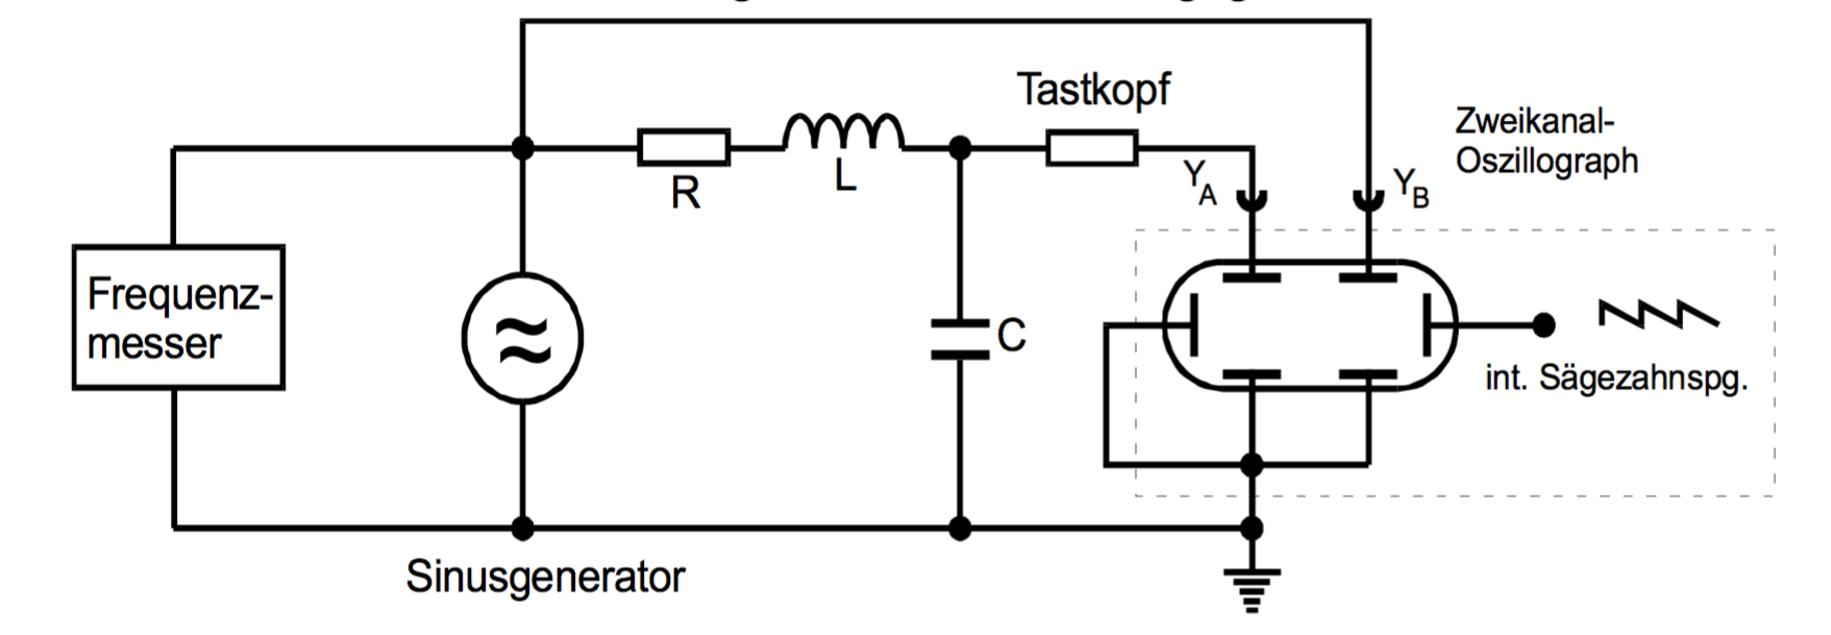
\includegraphics[width = \textwidth]{Schaltungcd.pdf}
  \caption{Schaltung zur Bestimmung von $U_C(\omega)$ und $\varphi(\omega)$ \cite{anleitung}.}
  \label{fig:schaltcd}
\end{figure}

Die Werte für $C$ und $L$ sind die Selben wie Kapitel \ref{sec:durchgedschw}.
Der Widerstand hat den Wert $R = \SI{67.2 \pm 0.2}{\ohm}$.

Die Spannungsquelle liefert in diesem Fall eine Sinusspannung und hat
den Innenwiderstand $R_{\text{i,sinus}} = \SI{50}{\ohm}$.

Nun werden die Messwerte aufgenommen. Die Frequenz kann an einem Frequenzmesser
abgelesen werden. Die Phase zwischen den beiden auf dem Oszilloskop zu erkennenden
Kurven kann aus dem Abstand der Nulldurchgänge errechnet werden, deshalb wird dieser
abgelesen und notiert. Die Spannung des Kondensators kann vom Osziilloskop
durch die Funktion $measure$ bestimmt werden.

In der Nähe der Resonanzfrequenz $\omega_{\text{res}}$ muss wesentlich
genauer gemessen werden, da die Werte dort stärkere Änderungen zeigen.
